% mc.tex

%\documentclass[extra,referee]{gji}
\documentclass[extra]{gji}
\usepackage{timet}
\usepackage{graphicx}

\title[Monte Carlo method for 1D velocity determination]
  {Monte Carlo method for coupled locations and 1D velocity
  determinations: ´Minimum´ models whith constant velocity 
  gradient layers
   }
\author[E. Kjartansson, I.Th. Bjarnason and H.M. Gheymasi] 
{Einar Kjartansson$^1$, Ingi Th. Bjarnason$^1$ and Hamzeh Mohammadi Gheymasi$^1$\\
$^1$ Institute of Earth Sciences, Science Institute, University of Iceland, Reykjavík, Iceland }
%\date{Received 1998 December 18; in original form 1998 November 22}
%\pagerange{\pageref{firstpage}--\pageref{lastpage}}
%\volume{219}
%\pubyear{2019}

%\def\LaTeX{L\kern-.36em\raise.3ex\hbox{{\small A}}\kern-.15em
%    T\kern-.1667em\lower.7ex\hbox{E}\kern-.125emX}
%\def\LATeX{L\kern-.36em\raise.3ex\hbox{{\Large A}}\kern-.15em
%    T\kern-.1667em\lower.7ex\hbox{E}\kern-.125emX}
% Authors with AMS fonts and mssymb.tex can comment out the following
% line to get the correct symbol for Geophysical Journal International.
\let\leqslant=\leq

\newtheorem{theorem}{Theorem}[section]
\bibliographystyle{gji}

\begin{document}

\label{firstpage}

\maketitle


\begin{summary}
% This guide is for authors who are preparing papers for
% \textit{Geophysical Journal International} using the
% \LaTeXe\ document preparation system and the GJI class file.
Ray-tracing through a one dimensional earth model consisting of layers of constant
velocity gradients, and continuous values across layers, is used to evaluate and improve
velocity models used for processing of micro erthquake data in Iceland.
Iterative Monte Carlo method is used to estimate the velocity values at boundaries between
layers with constant vertical velocity gradient, by searching for the velocity function that 
minimizes the residuals for observed arrival times for both P and S phases of micro earthquakes.
P and S velocities may be determined simultaneously.
S wave data are given similar weigths as P wave data.
Earthquakes are relocated for each iteration, the number of earthquakes used is typically in the
range from a few hundred to a few thousand.
The velocity functions are constraned so that the gradient can not increase with depth. This
ensures that traveltime curves are single valued and there is no focusing of rays.
\end{summary}

\begin{keywords}
-- seismic velocity function -- Monte Carlo -- Metropolis -- Ray tracing 
-- SISZ 
% \LaTeXe\ -- b"gji.cls"\ -- sample text -- user guide.
\end{keywords}

\section{Introduction}

The complex tectonic environment in Iceland is
a result of interaction between the relatively stable Icelandic hotspot
and the Mid-Atlantic Ridge, spreading at a rate of 1.9 cm/yr and 
drifting westward.
Manifestations of the ridge on land
are offset, oblique spreading segments. Two transform zones, 
the South Iceland Seismic Zone
(SISZ) and the Tjornes fracture zone, connect
the volcanically active segments.
The SISZ is essentially a left-lateral transform zone where the mid-Atlantic
rifting shifts from the Reykjanes Ridge and the Western Volcanic Zone, to
the Eastern Volcanic Zone in Iceland. Although the orientation of the
transform is east-west, most earthquakes are on faults oriented
north-south.


\begin{table}
\caption{SIL velocity model}
	\begin{center}
\begin{tabular}{ccc}
depth & P velocity & S velocity \\
(km) & (km/s) & (km/s) \\
0.00 & 3.53 & 1.98 \\
1.00 & 4.47 & 2.51 \\
2.00 & 5.16 & 2.90 \\
3.00 & 5.60 & 3.15 \\
4.00 & 5.96 & 3.35 \\
6.00 & 6.50 & 3.65 \\
9.00 & 6.73 & 3.78 \\
20.00 & 7.20 & 4.04 \\
32.00 & 7.40 & 4.16 \\
90.00 & 8.00 & 4.49 \\
	\end{tabular}
\end{center}

The SIL velocity model consist of layers where the vertical velocity gradient
is constant with in each layer, and velocity values are continous across layers
boundaries.

\end{table}

Historical records show
that larger earthquakes in the SISZ tend to cluster in
time. More than 30 destructive earthquakes in
the area have been documented since AD 1164,
either as single events, or more commonly as sequences 
of two or more magnitude 6-7 earthquakes over a 
period of days to a few years 
\citep{pe91}.
These earthquake sequences have recurred every 45-112
years 

Micro earthquake data has been recorded digitally in Iceland since 1990,
starting in the South Iceland Lowlands (SIL) region \citep{sil99}.
The network started with 
eight stations in SIL regions that were in operation by end of 1991.
Locations of the original stations are shown in Figure 2 as orange triangles.
Stations added later are shown as yellow triangles.
All SIL stations recored three components, sampled 100 times per seconds. 


\subsection{SIL model}

Routine processing of earthquake data is generally performed using one
dimensional earth models where the seismic velocities depend only on
depth. In Iceland the Icelandic Meteorological Office (IMO), which runs the
national earthquake network, uses one velocity model for routine
processing of most digital microearthquake data. 

It was originally based on
observations in the South Iceland Lowlands \citep{ib93}, and is refered to as the
SIL velocity 
model \citep{rs93}.

\begin{figure*}
%	\begin{minipage}{17cm}
	\figbox*{}{}{
		\includegraphics{tp.pdf} }
\caption{This figure shows ray paths throught the SIL model, from a source at
the surface, that turn at depths between 1550 and 6950 meters. Also
shown is velocity as a function of depth and reduced travel time (6.5
km/s). The figure shows that even for rays that are uniformly spaced
with 100 m separation between penetration depths, the spacing of
horizontal distances varies considerably. This effect is particularly
prominent for rays that turn at depths just above and below the
boundary at 6 km depth. The horizontal distance (offset) travelled by
a P wave that turns at 6 km depth is 29.9 km. In Figure 1 there are 13
rays in the distance range of 25 - 30 km but only one in the range of
30 - km. This abrupt change in ray density is caused by an abrupt
drop in the velocity gradient in the SIL model.
	}
%\end{minipage}
\end{figure*}
\begin{figure*}
\figbox*{}{}{
	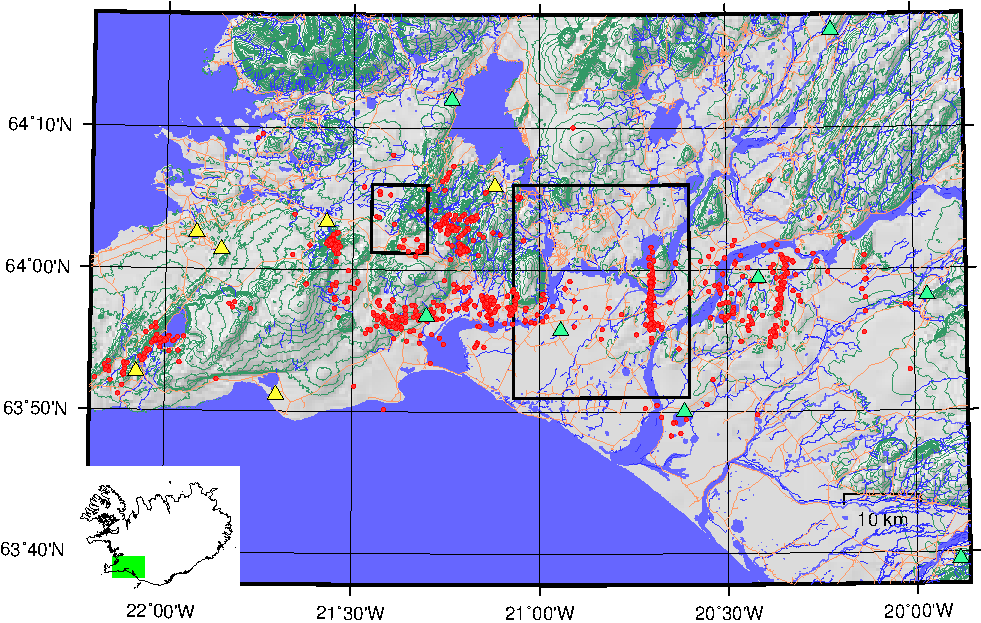
\includegraphics{sl2007-map.pdf}
	}
	\caption{
Map of the South Iceland seismic zone (SISZ). Location of seismograp stations are shown as yellow triangles. Red dots show location of selected
earthquakes from the period from january 1 2007 to april 30 2008, that were 
used to compute a mimimum velocity model.
		}
\end{figure*}

\begin{figure}
	\figbox*{}{}{
	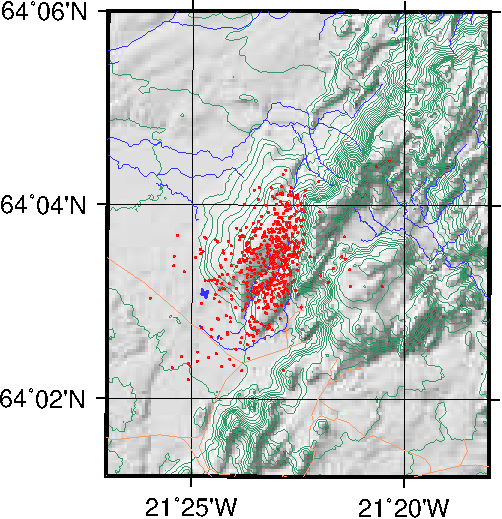
\includegraphics{hmE2011-map.pdf}
	}
	\caption{
		Map of Húsmuli region.
		}
\end{figure}

\begin{figure}
	\figbox*{}{}{
	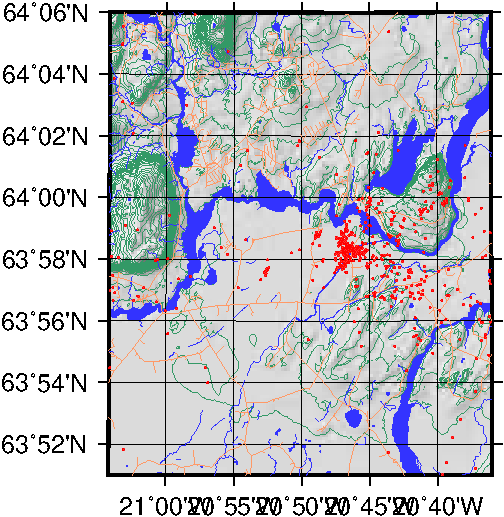
\includegraphics{skeidF-map.pdf}
	}
	\caption{
		Map of Hestfjall region.
		}
\end{figure}

\begin{figure}
	\figbox*{}{}{
	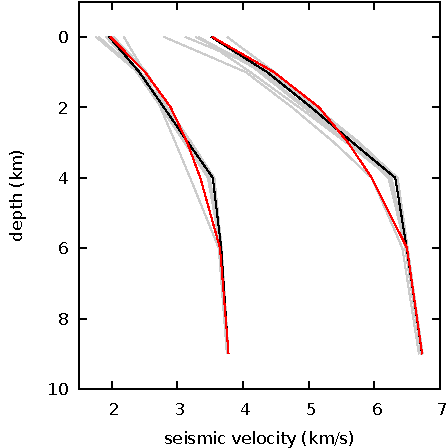
\includegraphics{sl2007-vel.pdf}
	}
	\caption{
		Velocity functions for SISZ.
		}
\end{figure}

\begin{figure}
	\figbox*{}{}{
	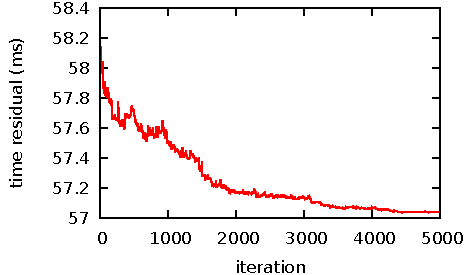
\includegraphics{sl2007-conv.pdf}
	}
	\caption{
		Convergence for SISZ.
		}
\end{figure}


\begin{figure}
	\figbox*{}{}{
	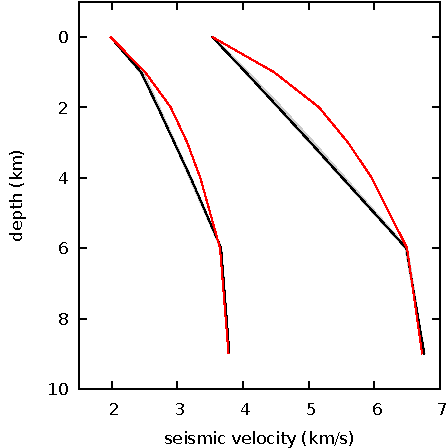
\includegraphics{hmE2011-vel.pdf}
	}
	\caption{
		Velocity functions for Husmuli.
		}
\end{figure}

\begin{figure}
	\figbox*{}{}{
	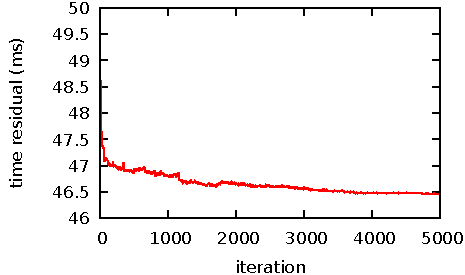
\includegraphics{skeidF-conv.pdf}
	}
	\caption{
		Convergence for Hestfjall region
		}
\end{figure}

\begin{figure}
	\figbox*{}{}{
	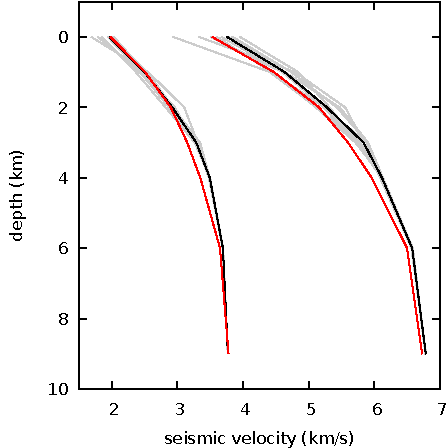
\includegraphics{skeidF-vel.pdf}
	}
	\caption{
		Velocity functions for Hestfjall region
		}
\end{figure}

\begin{figure}
	\figbox*{}{}{
	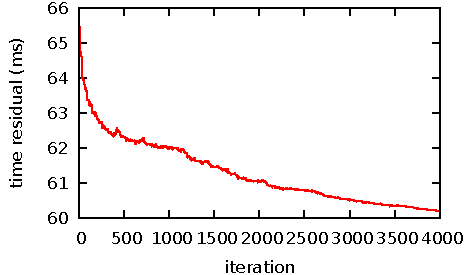
\includegraphics{hmE2011-conv.pdf}
	}
	\caption{
		Convergence for Husmuli
		}
\end{figure}




For 1-D velocity structure where velocity depends only on depth,
rays can be described using a ray parameter
defined by $ p=sin(u)/v $ where u is the angle of the ray relative to the
vertical and v is velocity. It follows from Snell's law, that the ray
parameter is constant for a given ray \citep{telf}.
When velocity increases
monotonically with depth, z, the maximum depth for the ray, where it
turns, can be determined by finding the depth where the velocity is
equal to 1/p. In a medium with a constant velocity gradient, the rays
are arcs of a circle. If the velocity is expressed as $v = a + bz$, then the
center of the circle is where $z = -a/b$.


A increase in velocity gradent at some depth will cause rays to cross, resulting in 
focusing and a triplication in 
traveltime versus distance.

We have  used ray-tracing to evaluate and improve the one-
dimensional velocity model. The iterative Monte Carlo (MC) method is used
to estimate velocity values, at boundaries between layers as described
above, by searching for the velocity function that minimizes the
residuals for observed arrival times for both P and S phases of micro
earthquakes.
MC methods utilize a random search through model space to find a
optimum solution. We use the root mean square of the time
residuals for each observed phase as a measue of the quality of the
trial solutions. Simulated annealing (MCSA) is a variation of the MC
method where the trial solutions are sometimes accepted even though
the quality declines \citep{menke13}.
We start with the SIL model and determine P and S velocities
simultaneously, i.e. the ratio beetween the velocities of P and S waves
is not constrained in the inversion. Weights proportional to P and S
wave velocities are applied to P and S wave observations. We show
results where velocity values for depths of 1,2,3,4,6 and 9 km were
determined using the MCSA method. At other depths the values from
the SIL model are used unchanged. The earthquakes are relocated for
each iteration.The number of earthquakes used is typically in the
range from a few hundred to a few thousand. The velocity functions
are constrained with gradients that decrease with depth. This ensures
that the travel-time curves are single valued and without any focusing
of rays.


\bibliography{mc}

\bsp % ``This paper has been produced using the Blackwell
     %   Publishing GJI \LaTeXe\ class file.''

\label{lastpage}


\end{document}
